\documentclass{beamer}

\usepackage[utf8]{inputenc}
\usepackage[spanish]{babel}
\usepackage{url}

% Más temas en
% http://deic.uab.es/~iblanes/beamer_gallery/index_by_theme.html
%\usetheme{Berlin}
%\usetheme{Copenhagen}
\usetheme{Warsaw}
%\usetheme{Darmstadt}

\setbeamercovered{transparent} %Items ocultos transparentes

\setbeamertemplate{background}{
  \rule{0pt}{.95\paperheight}%
  \hspace*{.98\paperwidth}%
  \makebox[0pt][r]{
\includegraphics[width=1.5cm]{fig/logo_fifa}}}

\title{Taller de Python}
\subtitle{Presentación}
\author{FIFA}
\institute[FIFA]{Federación Interestudiantil de Física Argentina}
\date{17 de abril de 2018}



%\AtBeginSubsection[]
%{
%  \begin{frame}<beamer>{Outline}
%    \tableofcontents[currentsection,currentsubsection]
%  \end{frame}
%}

% Let's get started
\begin{document}

\begin{frame}
  \titlepage
  
    \begin{figure}
    \centering
    
\includegraphics[width=0.4\textwidth]{fig/python-logo.png}
    \end{figure}

\end{frame}

%----------------------------------------------------------------------------------------------------------

\section{Presentación}

\subsection{¿Quiénes somos?}
\begin{frame}
\frametitle{¿Quiénes somos?}
    Somos la FIFA (Federación Interestudiantil de Física de Argentina),
filial Buenos Aires. Un grupo de estudiantes de Física de acá, de
Exactas UBA, que se junta para organizar actividades varias
(churreadas, congresos, fiestas, cine-debate, ciclos de charlas,
QNTT, etc), entre ellas este taller.
\end{frame}

\begin{frame}
¿Estudiás Física? Anotate en el grupo de mails, enterate de todas
las novedades y actividades, y encontrá un lugar para tus dudas
académicas, burocráticas y de cualquier otra cosa.
Mandá un mail a \textit{estufis@googlegroups.com}.
    
\end{frame}

\section{Introducción}
\subsection{¿Qué es programar?}
\begin{frame}{¿Qué es programar?}
    Programar es dar una lista de tareas concretas a la computadora
para que haga. Esencialmente, una computadora sabe:
\begin{itemize}
    \item Leer datos
    \item Escribir datos
    \item Transformar datos
\end{itemize}
\end{frame}

\begin{frame}{El proceso de la programación}
        \begin{figure}
    \centering
    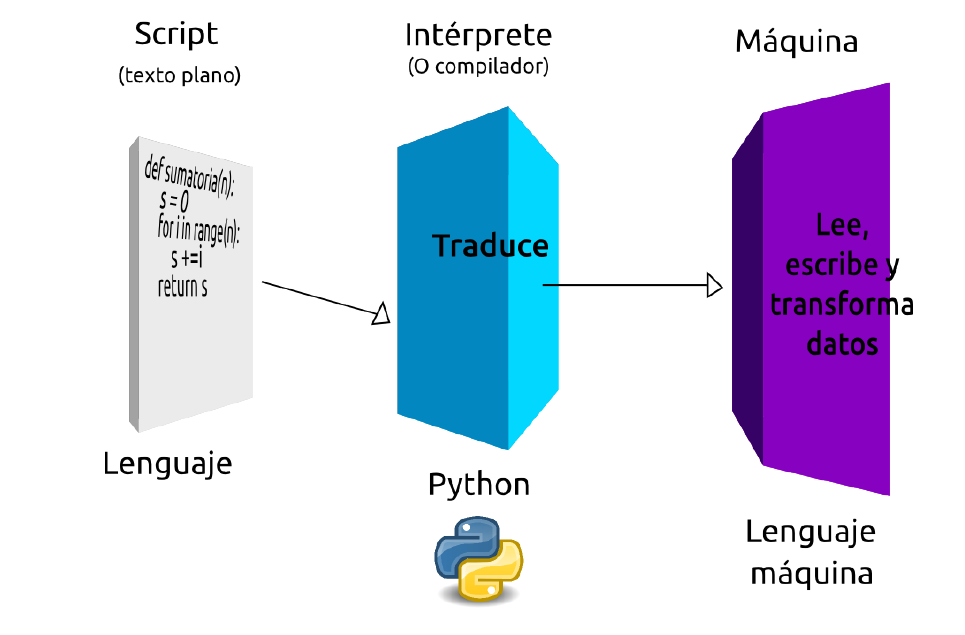
\includegraphics[width=\textwidth]{fig/programar.png}
    \end{figure}
\end{frame}

\begin{frame}{¿Para qué sirve programar?}

Como físicos, programar nos sirve para
    \begin{itemize}
        \item Resolver ``los ejercicios estrella" de las guías (de resolución
numérica)
\item Hacer simulaciones (Física computacional)
\item Hacer adquisición, procesamiento, análisis y gráfico de datos de
laboratorio
    \end{itemize}
\end{frame}

\begin{frame}{¿Qué es Python?}
Python es el lenguaje en el cual escribimos nuestro script. Es un
lenguaje interpretado, esto significa que cada línea es leída y
ejecutada una por una. Tiene diferentes versiones, en este taller usaremos la
versión 3.x, pero también existe la 2.7 que está cayendo en desuso.
    
\end{frame}


\subsection{Recursos}

\begin{frame}{¿Qué es la terminal?}
    Es una ventana con el intérprete. Los que están en Linux prueben
con \textbf{Ctrl+Alt+T} y escriban \textbf{ipython}. Luego escriban \textit{print ’Hola
mundo’}
        \begin{figure}
    \centering
    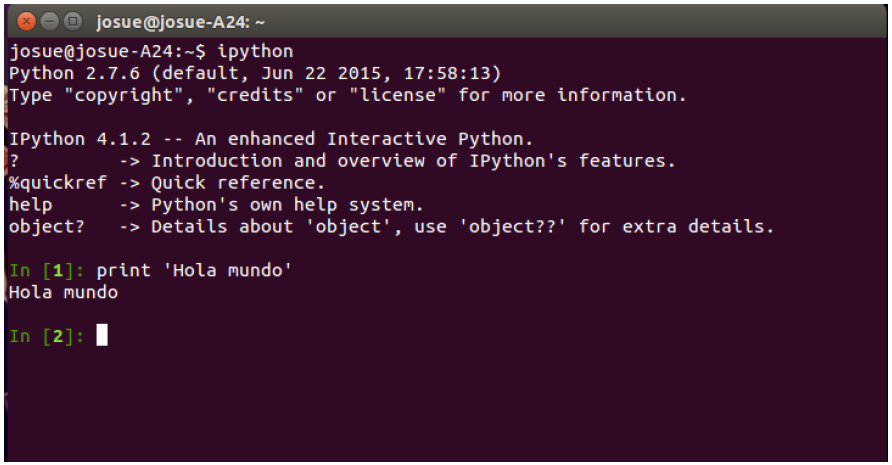
\includegraphics[width=\textwidth]{fig/terminal_HolaMundo.png}
    \end{figure}
    
\end{frame}

\begin{frame}{¿Cómo hacemos un script?}
    Abran un editor de texto plano. En Windows, block de notas o
Wordpad. En Linux, gedit (desde terminal, gedit).
        \begin{figure}
    \centering
    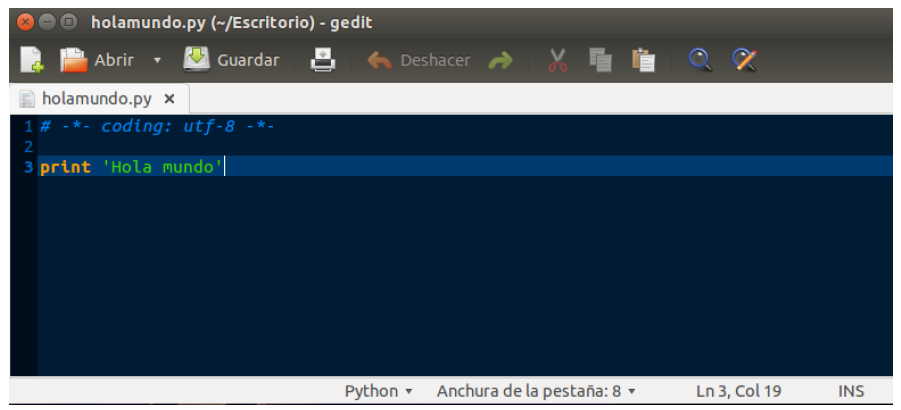
\includegraphics[width=\textwidth]{fig/script.png}
    \end{figure}
\end{frame}

\begin{frame}{¿Cómo lo ejecutamos?}
    Desde una terminal, \textit{python holamundo.py}
        \begin{figure}
    \centering
    \includegraphics[width=\textwidth]{fig/ejecutar_script.png}
    \end{figure}
\end{frame}

\begin{frame}{¿Hay algo más cómodo?}
    ¡Sí! El IDE \textbf{Spyder}
        \begin{figure}
    \centering
    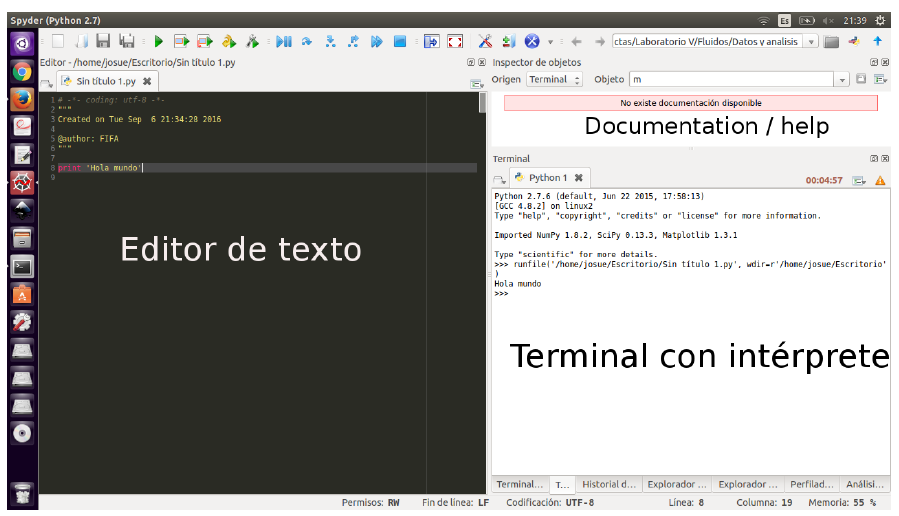
\includegraphics[width=\textwidth]{fig/imagen_Spyder.png}
    \end{figure}
\end{frame}

\section{Lo que sigue}

\begin{frame}{Orientándonos}

\begin{enumerate}
    \item Variables y operaciones
  \begin{itemize}
      \item Enteros
      \item Floats
      \item Strings
    \item Listas y tuplas
    \item Booleans
  \end{itemize}  

\item  Control de flujo (if, for, while)
\item  Funciones
\item  Bibliotecas
\end{enumerate}

\end{frame}

\end{document}
